\subsubsection{Enhance}

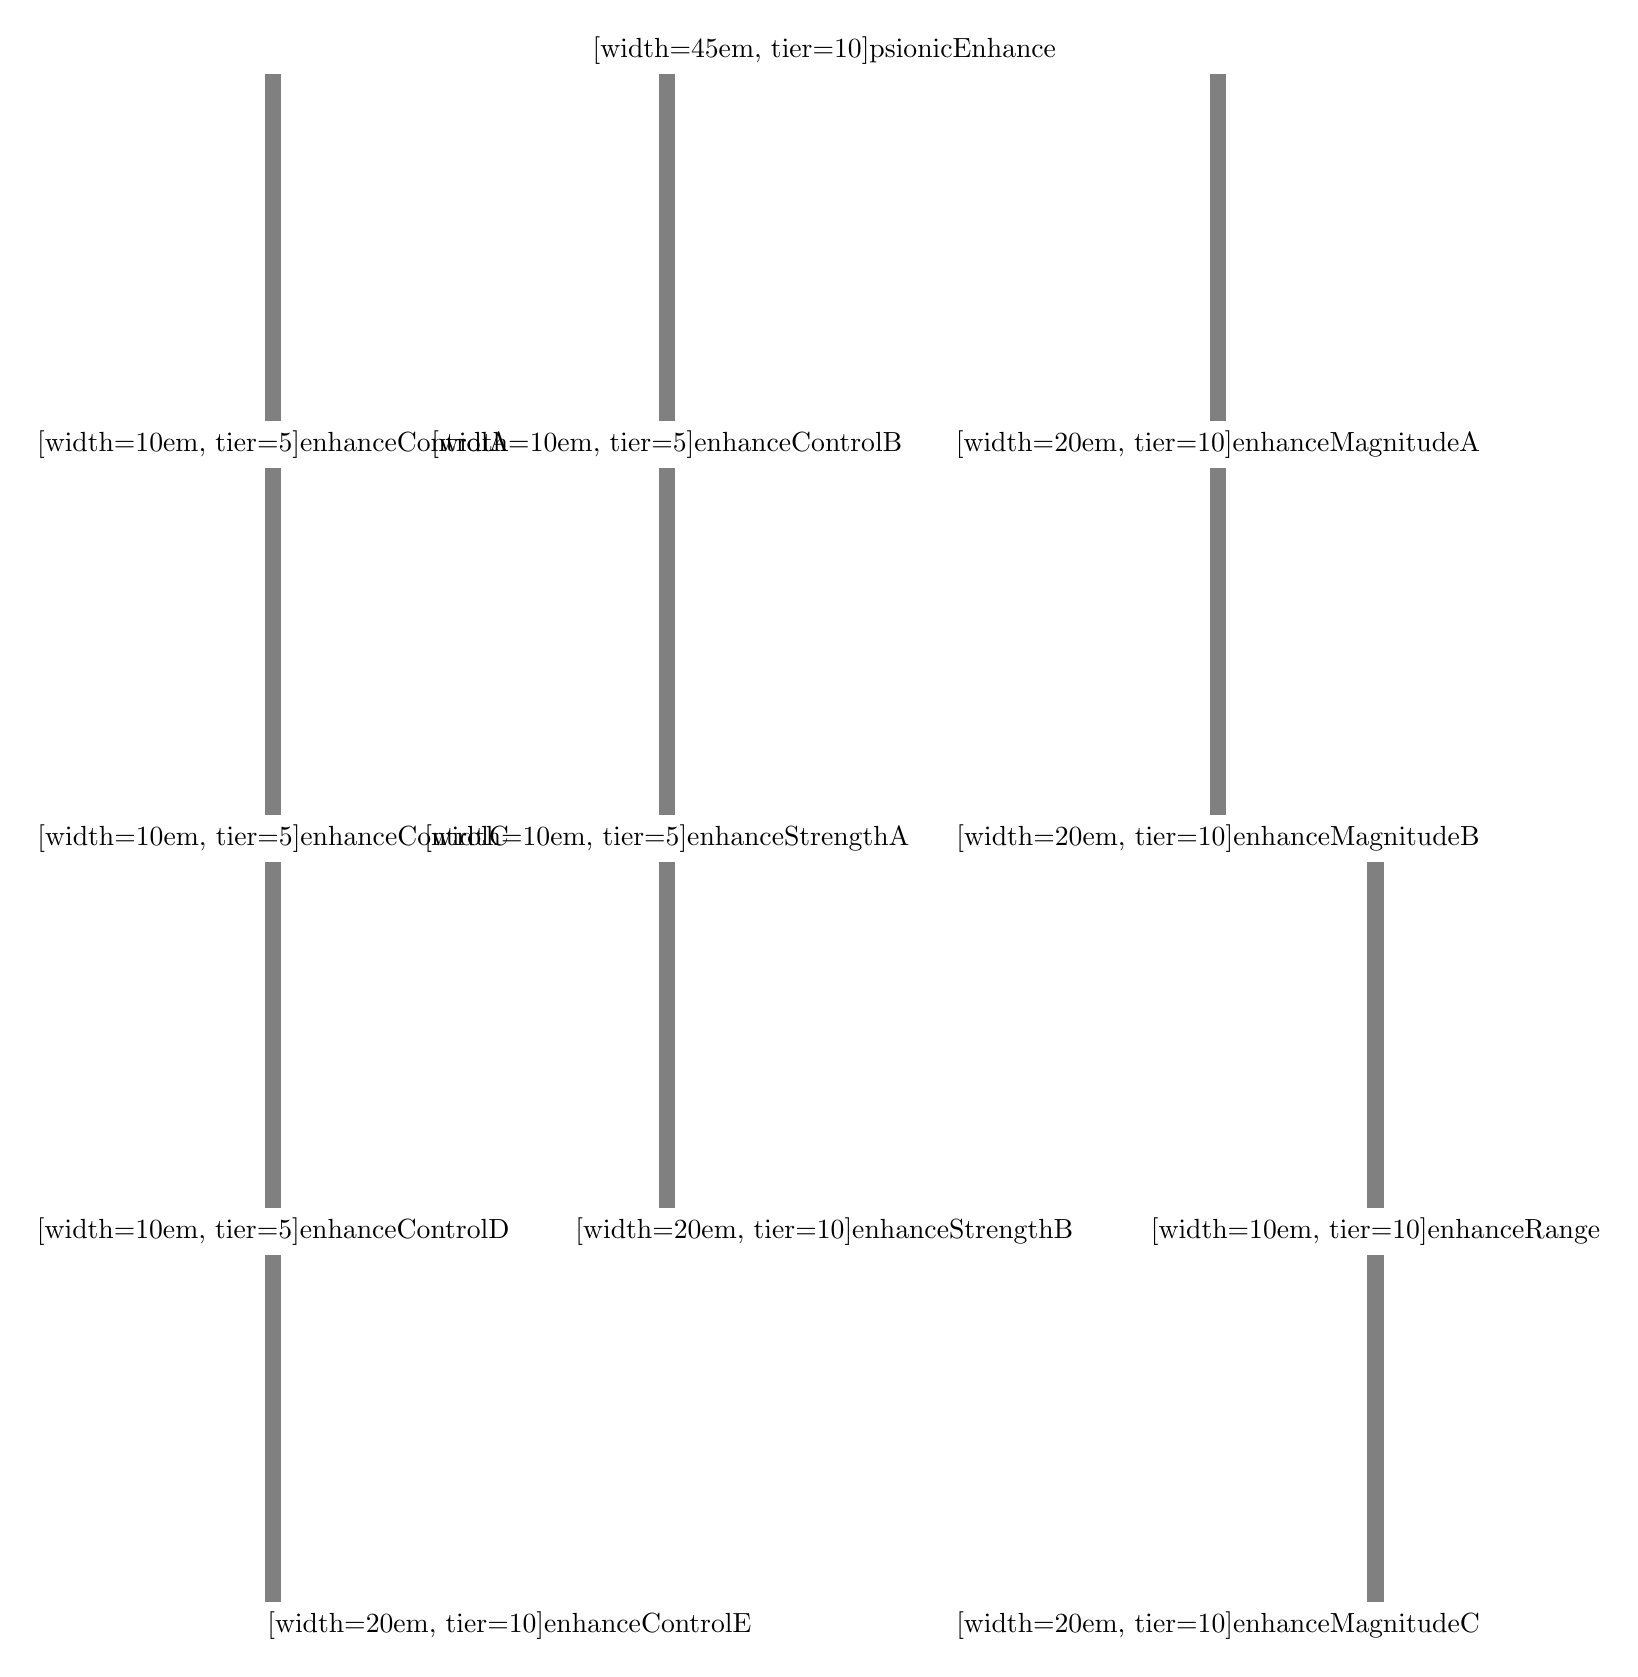
\begin{tikzpicture}
    \draw ( -13,  -2) node(pr){\TalentBox[width=45em, tier=10]{psionicEnhance}};
    \draw ( -20,  -7) node(aa){\TalentBox[width=10em, tier=5]{enhanceControlA}}
          ( -15,  -7) node(ab){\TalentBox[width=10em, tier=5]{enhanceControlB}}
          (  -8,  -7) node(ad){\TalentBox[width=20em, tier=10]{enhanceMagnitudeA}}
          ( -20, -12) node(ba){\TalentBox[width=10em, tier=5]{enhanceControlC}}
          ( -15, -12) node(bb){\TalentBox[width=10em, tier=5]{enhanceStrengthA}}
          (  -8, -12) node(bd){\TalentBox[width=20em, tier=10]{enhanceMagnitudeB}}
          ( -20, -17) node(ca){\TalentBox[width=10em, tier=5]{enhanceControlD}}
          ( -13, -17) node(cc){\TalentBox[width=20em, tier=10]{enhanceStrengthB}}
          (  -6, -17) node(cd){\TalentBox[width=10em, tier=10]{enhanceRange}}
          ( -17, -22) node(db){\TalentBox[width=20em, tier=10]{enhanceControlE}}
          (  -8, -22) node(dd){\TalentBox[width=20em, tier=10]{enhanceMagnitudeC}}
    ;

    \tikzstyle{bar}=[gray,-,>=stealth, line width=6pt]

    \draw [bar] (aa) -- (aa |- pr.south);
    \draw [bar] (ab) -- (ab |- pr.south);
    \draw [bar] (ad) -- (ad |- pr.south);
    \draw [bar] (aa) edge (ba);
    \draw [bar] (ab) edge (bb);
    \draw [bar] (ad) edge (bd);
    \draw [bar] (ba) edge (ca);
    \draw [bar] (bb) -- (bb |- cc.north);
    \draw [bar] (cd) -- (cd |- bd.south);
    \draw [bar] (ca) -- (ca |- db.north);
    \draw [bar] (cd) -- (cd |- dd.north);
\end{tikzpicture}
